\subsection{Bazy danych}

\begin{definition}
    \textbf{Baza danych} to zorganizowany zbiór powiązanych ze sobą informacji (danych).
\end{definition}

\begin{definition}
    \textbf{System zarządzania bazą danych} (database-management system, DBMS) to opragramowanie,
    umożliwiające dostęp do danych i zarządzanie nimi. Głównym celem SZBD jest zapewnienie takiego sposobu
    przechowywania i przetwarzania informacji, który jest jednocześnie wygodny, wydajny i bezpieczny.
\end{definition}

\begin{definition}
    \textbf{Systemem bazy danych} (database system) nazwiemy bazę danych wraz z systemem zarządzania bazą danych.
\end{definition}

Przykłady zastosowań baz danych:

\begin{itemize}
    \item Bankowość: obsługa klienta, zarządzanie kontami, transakcje płatnościowe, naliczanie odsetek...
    \item Sklepy internetowe: informacje o produktach i klientach, tworzenie koszyków, realizacja zamówień, przyznawanie rabatów...
    \item USOS: informacje o studentach i pracownikach uniwersytetu, harmonogram zajęć, protokoły, ankiety...
    \item ResearchGate: informacje o naukowcach i publikacjach, rekomendacje, oferty pracy w branży naukowej...
    \item OpenStreetMap: mapy, planowanie przejazdu, zdjęcia lotnicze, tworzenie map...
\end{itemize}

Przykłady wielkich systemów baz danych:

\begin{itemize}
    \item Biblioteka Kongresu Stanów Zjednoczonych \\
            ponad 38 milionów książek, 14 milionów zdjęć, 5,5 miliona map, 70 milionów manuskryptów, łącznie ponad 167 milionów dokumentów
    \item Wielki Zderzacz Hadronów (LHC) \\
            przetwarzanie gigantycznej ilości danych, obecnie ok. 90 petabajtów rocznie
    \item LexisNexis \\
            system informacyjny służący do gromadzenia, systematyzowania, przetwarzania i wyszukiwania informacji prawnych \\
            250 terabajtów informacji o Amerykanach
    \item The World Data Centre for Climate \\
            220 terabajtów danych dostępnych w Internecie, 110 terabajtów symulacji klimatycznych, ponad 8 petabajtów danych przechowywanych na dyskach
\end{itemize}

\begin{definition}
    \textbf{Płaski plik} to prosta organizacja danych, będąca sekwencją zapisów nieposiadających wewnętrznej ani zewnętrznej struktury.
\end{definition}

Aby wyszukać w nim rekord, należy przejrzeć plik od początku.
Tak zapisywane były dane w czasach, gdy nie było jeszcze komercyjnych systemów baz danych.

Przykład: pliki \textbf{CSV} (comma-separated values), oddzielne dla różnych typów obiektów. Służą do zapisywania danych w plikach tekstowych i mogą być przydatne
w przenoszeniu danych.

\subsection{Czego oczekujemy od SZBD?}

System zarządzania bazą danych powinien zapewniać:
\begin{itemize}
    \item przechowywanie i przetwarzanie gigantycznych ilości danych
    \item trwałość danych
    \item bezpieczeństwo
    \item obsługę wielu użytkowników
    \item wygodę
    \item wydajność
    \item niezawodność
    \item spójność danych
\end{itemize}

W roku 1970 Ted Codd wprowadza model relacyjny, publikując artykuł \textbf{A Relational Model of Data for Large Shared Data Banks}.

Proponuje trzynaście postulatów, wśród których są następujące.

\begin{enumerate}
    \item Dane powinny być przechowywane w prostych strukturach
    \item Dostęp do nich powinien być możliwy za pomocą języka wysokiego poziomu
    \item Dane powinny być niezależne zarówno w warstwie fizycznej, jak i logicznej
\end{enumerate}

\subsection{Podział systemów baz danych}

Podziału systemów bazodanowych możemy dokonać ze względu na różne kryteria:
\begin{itemize}
    \item \textbf{Model danych} \\
    Co właściwie chcemy reprezentować?
    Jaka jest struktura naszych danych?
    Jakie są między nimi zależności?
    Jakie ograniczenia musimy zamodelować?
    \item \textbf{Cel wykorzystania} \\
    Jakie operacje będą wykonywane?
    Czy będziemy dokonywać częstych zmian w bazie czy może dominować będą odczyty?
    \item \textbf{Wolumen danych i liczba użytkowników} \\
    Czy nasza baza będzie obsługiwana przez jednego użytkownika czy przez wielu?
    Czy wszystkie dane dają się zapisać w jednym, stosunkowo niewielkim pliku, czy może chodzi o terabajty informacji?
    \item \textbf{Sposób przechowywania danych} \\
    Czy cała baza będzie znajdować się na jednym urządzeniu czy będzie istnieć fizycznie na wielu maszynach?
\end{itemize}

Podział ze względu na \textbf{ilość danych}:
\begin{itemize}
    \item \textbf{Wbudowane systemy zarządzania bazami danych} (embedded DBMS) \\
    Obsługują bardzo małe bazy, są wbudowane w aplikację, sprawdzają się w przypadku lokalnych aplikacji wykorzystywanych przez jednego użytkownika, działają szybko i wydajnie, nie nadają się w sytuacji, gdy dokonywanych jest wiele zapisów.
    \item \textbf{Hurtownie danych} (data warehouse) \\
    Są to rozbudowane bazy danych przechowujące olbrzymie ilości danych, przeprowadzane operacje mają charakter analityczny, a nie transakcyjny.
\end{itemize}

Podział ze względu na \textbf{liczbę węzłów}:
\begin{itemize}
    \item \textbf{Bazy scentralizowane} \\
    Cechuje je wysoka przepustowość, większa dostępność, a także niewielkie opóźnienia, problemem jest zapewnienie bezpieczeństwa i odporności na manipulacje.
    \item \textbf{Bazy rozproszone} \\
    Zapewniają większą prywatność oraz bezpieczeństwo kosztem możliwego przeciążenia sieci i opóźnień transakcji.
\end{itemize}

\subsection{Główne cele stosowania baz danych}

\begin{definition}
    \textbf{Przetwarzanie transakcyjne} (OLTP, Online Transaction Processing): system wspomaga korzystanie z bazy danych przez wielu użytkowników, z których każdy odbiera względnie małą ilość danych i dokonuje odczytu lub niewielkich modyfikacji.
\end{definition}

\begin{definition}
    \textbf{Przetwarzanie analityczne} (OLAP, Online Analytical Processing): system wspomaga korzystanie z bazy danych przez niewielką liczbą użytkowników, który odbiera dużą ilość danych i dokonuje złożonych operacji analitycznych.
\end{definition}

\subsection{Typy modeli danych}

Istnieje wiele modeli danych, w tym między innymi:
\begin{itemize}
    \item relacyjny
    \item związków encji
    \item obiektowy
    \item NoSQL:
        \begin{itemize}
            \item klucz-wartość
            \item grafowy
            \item rodzina kolumn
            \item dokument
        \end{itemize}
    \item przestrzenny
    \item temporalny
    \item hierarchiczny
    \item sieciowy
\end{itemize}

\subsection{Poziomy abstrakcji danych}

Aby ułatwić użytkownikom korzystanie z systemu bazodanowego, dostęp do danych jest wielopoziomowy.

\begin{itemize}
    \item Najniższy poziom to \textbf{poziom fizyczny} (physical level), który określa, w jaki sposób dane są przechowywane na dysku oraz szczegóły implementacyjne struktur danych.
    \item Pośredni poziom to \textbf{poziom logiczny} (logical level), który określa, jakie dane znajdują się w bazie oraz jakie zachodzą między nimi związki. Już na tym etapie dla użytkownika nie są istotne szczegóły implementacyjne wykorzystywanych struktur.
    \item Najwyższy poziom to \textbf{poziom zewnętrzny} (view level), który określa sposób użycia bazy danych przez użytkowników końcowych. System może zapewniać różne widoki dla różnych użytkowników
\end{itemize}

\begin{figure}[H]
    \centering
    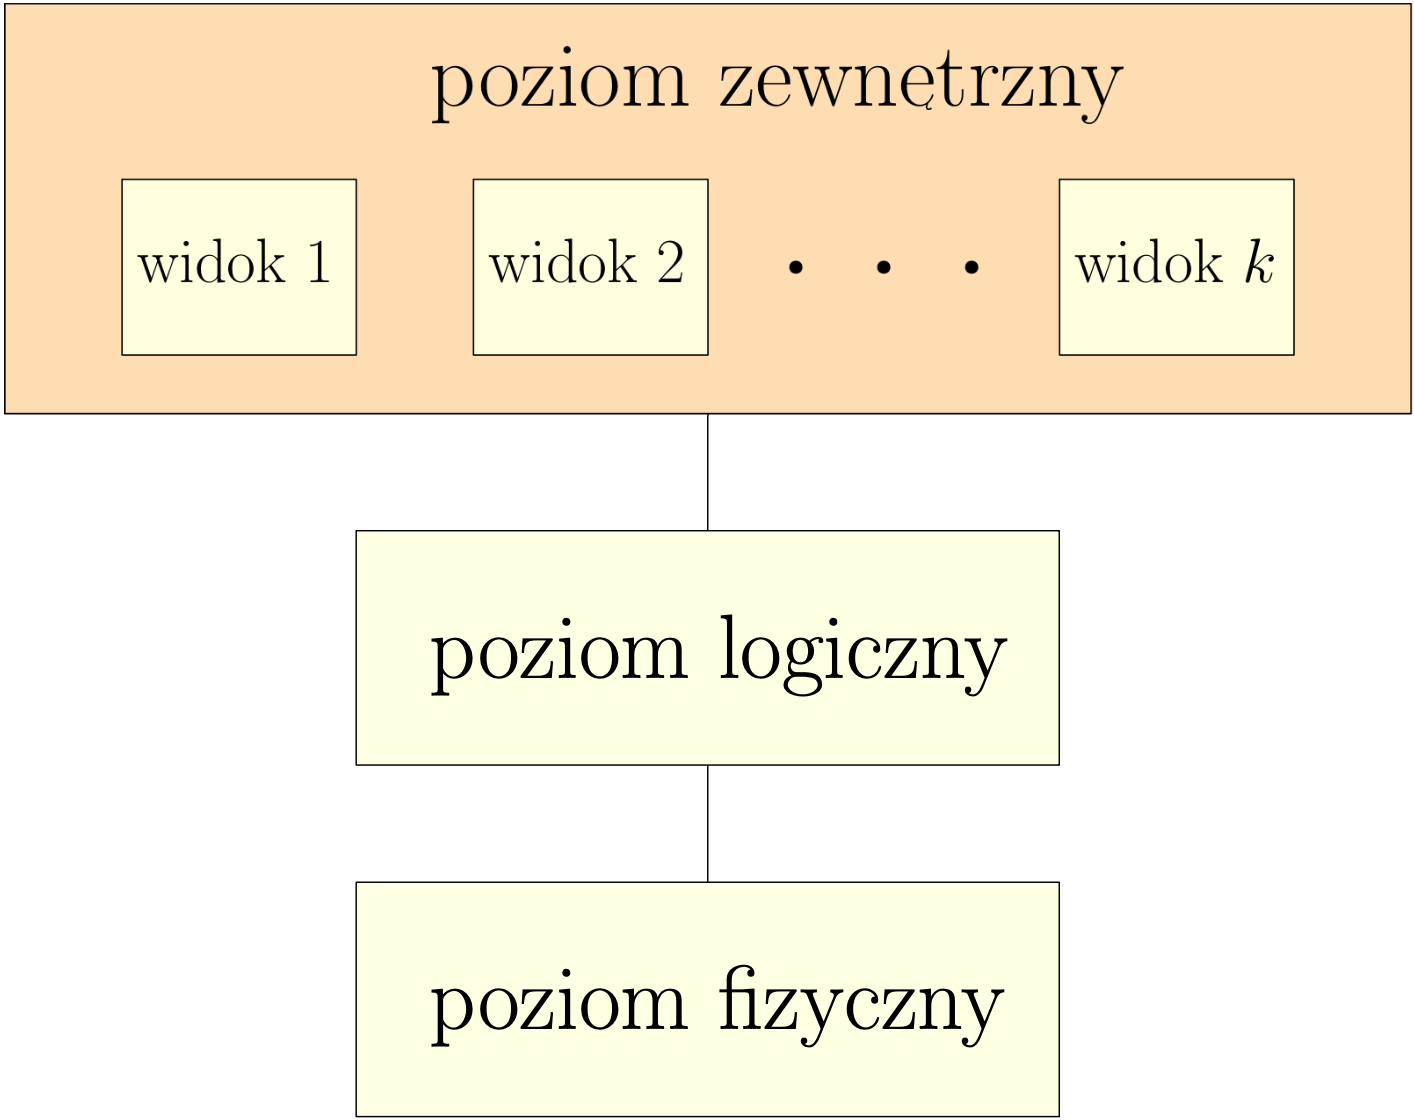
\includegraphics[scale=0.25]{images/podstawowe/poziomy-abstrakcji.png}
    \caption{Poziomy abstrakcji danych}
\end{figure}

\subsection{Schematy}

\begin{definition}
    \textbf{Stan} bazy danych to zbiór wszystkich danych w danej chwili.
\end{definition}

\begin{definition}
    \textbf{Schemat} bazy danych to opis ogólnej struktury bazy danych.
\end{definition}

\begin{definition}
    \textbf{Schemat fizyczny} to opis na poziomie fizycznym, w jaki sposób dane są przechowywane na dysku.
\end{definition}

\begin{definition}
    \textbf{Schemat logiczny} to opis na poziomie logicznym, jakie dane znajdują się w bazie oraz jakie zachodzą między nimi związki.
\end{definition}

\begin{definition}
    \textbf{Podschemat} to opis na poziomie zewnętrznym, jakie dane są dostępne dla konkretnego użytkownika, opis widoków bazy danych.
\end{definition}

\begin{figure}[H]
    \centering
    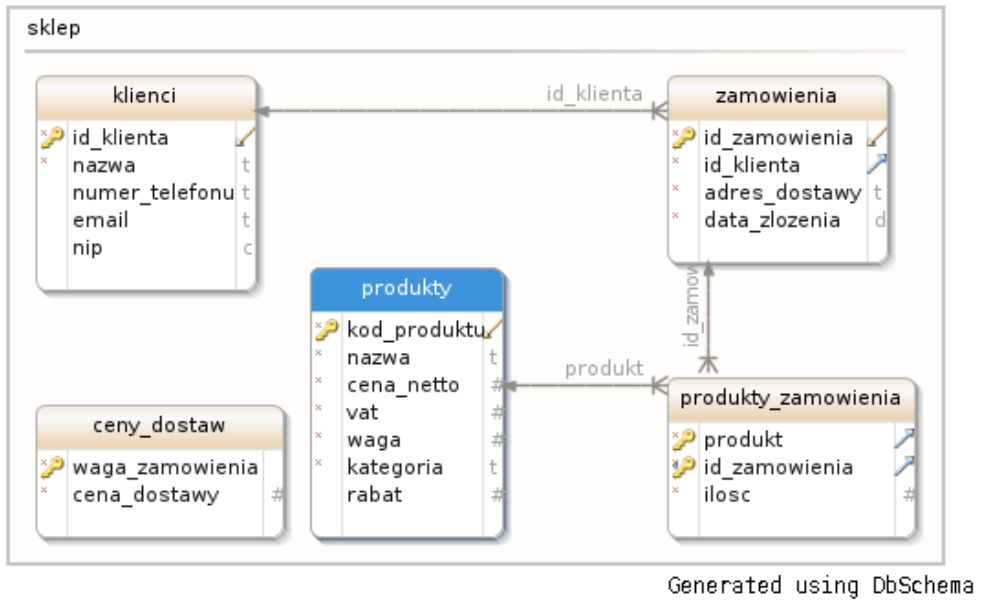
\includegraphics[scale=0.50]{images/podstawowe/schemat-logiczny.png}
    \caption{Przykład schematu logicznego}
\end{figure}

\subsection{Języki baz danych i SQL}

Interakcję z bazą danych zapewniają języki:

\begin{itemize}
    \item \textbf{Język definicji danych DDL} (Data Definition Language) \\
    Pozwala na tworzenie, modyfikowanie i usuwanie struktur danych.
    \item \textbf{Język manipulacji danych DML} (Data Manipulation Language) \\
    Pozwala na dodawanie, modyfikowanie i usuwanie danych.
    \item \textbf{Język zapytań danych DQL} (Data Query Language) \\
    Pozwala na wyszukiwanie danych.
    \item \textbf{Język kontroli transakcji TCL} (Transaction Control Language) \\
    Pozwala na zarządzanie transakcjami.
\end{itemize}

Zazwyczaj nie są to różne języki, a stanowią część jednego języka.
W przypadku relacyjnych baz danych jest to praktycznie zawsze \textbf{SQL} (Structured Query Language).

\textbf{SQL} jest deklaratywnym językiem wysokiego poziomu (tzn. specyfikuje strukturę wyniku, a nie sposób jego realizacji).

\subsubsection{DDL - Data Definition Language}

Język definicji danych służy do zdefiniowania schematu logicznego oraz określenia własności danych, takich jak dziedzina danych (typ, zakres długości, format) czy integralność referencyjna (utrzymanie powiązań między tabelami).

Najważniejsze polecenia DDL to: \texttt{CREATE}, \texttt{ALTER}, \texttt{DROP}.

\subsubsection{DML - Data Manipulation Language}

Język manipulacji danych służy do dodawania, modyfikowania i usuwania danych w bazie.

Najważniejsze polecenia DML to: \texttt{INSERT}, \texttt{UPDATE}, \texttt{DELETE}.

\subsubsection{DQL - Data Query Language}

Język zapytań danych służy do wyszukiwania danych w bazie.

W zakres języka wchodzi tylko jedno polecenie - \texttt{SELECT}.

\subsubsection{DCL - Data Control Language}

Język kontroli nad danymi służy do nadawania uprawnień użytkownikom do obiektów bazodanowych, przypisywania ról, zmieniania haseł.

Najważniejsze polecenia DCL to: \texttt{GRANT}, \texttt{REVOKE}.

\subsection{Fazy projektowania bazy danych}

Projektowanie bazy danych można podzielić na kilka faz:
\begin{itemize}
    \item \itextbf{Faza konceptualna}
    \item \itextbf{Faza logiczna}
    \item \itextbf{Faza fizyczna}
\end{itemize}

\subsubsection{Faza konceptualna}

Projektowanie bazy danych dotyczy głównie projektowania schematu. Początkowa faza zakłada zebranie informacji i specyfikację potrzeb i wymagań przyszłych użytkowników bazy.

Na podstawie analizy dotyczącej wymagań i funkcjonalności, niezależnie od szczegółów implementacyjnych, tworzy się model konceptualny.

W przypadku modelu relacyjnego należy:
\begin{itemize}
    \item ustalić występujące zbiory encji,
    \item ustalić występujące związki i ich typy,
    \item określić atrybuty poszczególnych encji i związków, podać dziedziny tych atrybutów,
    \item ustalić klucze relacji,
    \item zweryfikować otrzymany model pod kątem występowania redundancji oraz możliwości realizowania transakcji.
\end{itemize}

\subsubsection{Faza logiczna i fizyczna}

Kolejna faza polega na transformacji modelu konceptualnego w model logiczny.

W przypadku modelu relacyjnego na tym etapie należy:
\begin{itemize}
    \item wyznaczyć relacje odpowiadające encjom i związkom z modelu konceptualnego,
    \item znormalizować relacje,
    \item wyznaczyć więzy integralnościowe,
    \item w przypadku tworzenia oddzielnych modeli dla większej liczby użytkowników utworzyć model globalny.
\end{itemize}

Ostatni etap to implementacja bazy danych z uwzględnieniem relacji, organizacji plików, indeksów (czyli struktur danych stosowanych w celu efektywnego dostępu do danych), więzów integralnościowych i zagadnień związanych z bezpieczeństwem.

\subsection{Główne składowe SZBD}

Za wykonywanie poszczególnych zadań w obrębie SZDB odpowiedzialnych jest kilka modułów:
\begin{itemize}
    \item \textbf{Moduł zarządzania pamięcią}, wybierający właściwe dane z pamięci,
    \item \textbf{Moduł zarządzania zapytaniami}, analizujący zapytania i wybierający najlepsze strategie ich realizacji,
    \item \textbf{Moduł zarządzania transakcjami}, dbający o poprawność realizacji transakcji.
\end{itemize}

\subsubsection{Moduł zarządzania pamięcią}

Moduł zarządzania pamięcią dzieli się na następujące składowe:
\begin{itemize}
    \item \textbf{Modul zarządzania autoryzacją i integralnością danych},  sprawdzający, czy spełnione są wszystkie ograniczenia nałożone na dane oraz kontrolujący autoryzację użytkowników;
    \item \textbf{Moduł zarządzania plikami}, przechowujący dane o miejscu zapisania plików na dysku i struktury danych wykorzystywane do reprezentowania informacji przechowywanych na dysku;
    \item \textbf{Moduł zarządzania buforami}, odpowiedzialny za przekazywanie danych z dysku do pamięci operacyjnej i decyzje, które przechowywać w pamięci podręcznej.
\end{itemize}

Ponadto moduł ten tworzy pliki danych (przechowujące dane), słownik danych (przechowujący metadane o strukturze bazy) oraz indeksy.

\subsubsection{Moduł zarządzania zapytaniami}

Moduł zarządzania zapytaniami dzieli się na następujące składowe:
\begin{itemize}
    \item \textbf{Interpreter języka DDL}, interpretujący polecenia w języku definicji danych i zapisujący odpowiednie metadane w słowniku;
    \item \textbf{Interpreter języka DML}, tworzący plany zapytań dla polecenia w języku manipulacji danymi, wybierający optymalny plan i tłumaczący go na język niskiego poziomu;
    \item \textbf{Modul wykonujący zapytania}, realizujący niskopoziomowe instrukcje przekazywane przez kompilator DML.
\end{itemize}

\subsubsection{Moduł zarządzania transakcjami i ACID}

Moduł zarządzania transakcjami zapewnia poprawność przeprowadzenia transakcji.

Poprawność oznacza w tym wypadku:
\begin{itemize}
    \item \textbf{Niepodzielność} (ang. \textit{atomicity}) - transakcja jest albo przeprowadzona w całości, albo wcale,
    \item \textbf{Spójność} (ang. \textit{consistency}) - baza danych przechodzi z jednego spójnego stanu w drugi spójny stan,
    \item \textbf{Izolacja} (ang. \textit{isolation}) - czyli żadne dwie transakcje przetwarzane równocześnie nie wpływają wzajemnie na siebie,
    \item \textbf{Trwałość} (ang. \textit{durability}) - czyli po zakończeniu transakcji jej wynik nie zostanie utracony z powodu awarii systemu.
\end{itemize}

% Tutaj jeszcze można dodac o użytkownikach, ich uprawnieniach, rolach, itp.

\subsection{Podsumowanie}

\textbf{Zalety SZBD}:
\begin{itemize}
    \item kontrola redundancji,
    \item zabiezpieczenia przed nieautoryzowanym dostępem,
    \item wspólbieżność dostępu,
    \item trwałość danych, możliwość ich odzyskiwania i przechowywania kopii zapasowych,
    \item struktury i techniki pozwalające na efektywny dostęp do danych i ich przetwarzanie,
    \item reprezentacja złożonych zależności między danymi,
    \item ograniczenia integralnościowe,
    \item niezależność danych od działających na nich programów.
\end{itemize}

\textbf{Wady SZBD}:
\begin{itemize}
    \item początkowa inwestycja: zasoby ludzkie, architektura, czas,
    \item duża złożoność,
    \item koszty związane z zarządzaniem i konserwacją systemu.
\end{itemize}